\section{Introduction}
    There are various levels of autonomous vehicles (AV) depending on the degree of autonomy and in this work we focus on the security of the fully automated vehicles.. In this type of AV all aspects of the dynamic driving tasks, under all roadway and environmental conditions that can be managed by a human driver, are performed by the automated system, and this, potentially without driver present in the vehicle. However, automated vehicles can only work properly with accurate, reliable and trustworthy sensors. Figure 1 give us an overview of how an AV work.
    \newline
    Some example of AVs are the Stanford Shelley [1], AnnieWAY [2] and Google Driverless Car [3]. All of those cars use Light Imaging Detection and Ranging (LiDAR) to detect objects and camera for traffic sign recognition. These two sensors act together to influence the mission planning. When LiDAR detects an obstacle on the road, the mission is replanned to avoid that object. Resilience of AV sensors against attacks is a key challenge. Indeed, any attack that degrades sensor data can cause false driving reaction, leading potentially to accidents and fatalities [4]. For example, if camera is attacked, it can misread a speed limit sign, leading to unsafe driving conditions for the vehicle’s passengers. If a LiDAR detects a fake obstacle because of an attack and triggers an emergency brake, it will seriously alter traffic efficiency if it’s done for example in the highway. 
    \newline
    Furthermore, automated vehicles can communicate with each other and share information about the environment. Communication is not limited to communication between cars or to communication between cars and the infrastructure [5]. A cyber attack can be done with control technology tools that are embedded in AVs such as electrical window controls, which are now controlled by engine control units (ECUs) as embedded systems. The ECU is one of the most important parts of a vehicle [6]. An attacker can modify the programming code during design and implementation processing. This attack is done in order to corrupt or degrade hardware performance, or to destroy informations. In [7] was created a virus that could modify the messages delivered by the controller area network (CAN) bus. Upon successful capture of door locking messages, this virus was able to remotely lock a vehicle’s doors. Security issues involving the CAN bus, which connects to all the vehicle’s components, crate risks for drive safety and privacy. A cyber attacker can configure the settings, modify code, and implant viruses and malware [8][6].
    \newline
    The key contribution of this paper are:
    \begin{itemize}
        \item We present a detailed, accurate and updated overview about the state-of-art of AV safety issue and corresponding countermeasures;
        \item We describe almost all the possible attacks that could be done in AV because this type of work hasn't yet been done before in this way. In our knowledge, we are the first considering all of these scenarios, while other survey focus on only a small subset;
        \item We present also all the opened issue for researchers that aim to join this research field.
    \end{itemize}
    
    
    
    \begin{figure*}
        \centering
        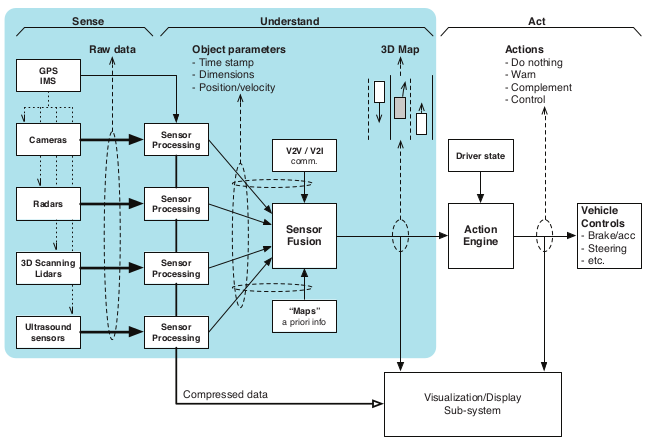
\includegraphics[width=.7\linewidth]{./files/Schermata da 2020-02-13 12-41-35.png}
        \caption{Autonomous vehicle overview.}
        \label{fig:AVoverview}
    \end{figure*}

